\documentclass[11pt]{article}
\usepackage{fullpage}
\usepackage{fancyhdr}

\usepackage{amsmath}
\usepackage{amssymb}
\usepackage{url}

\usepackage{listings}
\usepackage{color}
\lstset{language=Python,
        basicstyle=\footnotesize\ttfamily,
        showspaces=false,
        showstringspaces=false,
        tabsize=2,
        breaklines=false,
        breakatwhitespace=true,
        identifierstyle=\ttfamily,
        keywordstyle=\color[rgb]{0,0,1},
        commentstyle=\color[rgb]{0.133,0.545,0.133},
        stringstyle=\color[rgb]{0.627,0.126,0.941},
    }

\usepackage[pdftex]{graphicx}

% header
\fancyhead{}
\fancyfoot{}
\fancyfoot[C]{\thepage}
\fancyhead[R]{Daniel Foreman-Mackey}
\fancyhead[L]{Probabilistic Graphical Models --- Problem Set 5}
\pagestyle{fancy}
\setlength{\headsep}{10pt}
\setlength{\headheight}{20pt}

% shortcuts
\newcommand{\Eq}[1]{Equation (\ref{eq:#1})}
\newcommand{\eq}[1]{Equation (\ref{eq:#1})}
\newcommand{\eqlabel}[1]{\label{eq:#1}}
\newcommand{\Fig}[1]{Figure \ref{fig:#1}}
\newcommand{\fig}[1]{Figure \ref{fig:#1}}
\newcommand{\figlabel}[1]{\label{fig:#1}}

% commands
\newcommand{\pr}[1]{\ensuremath{p(#1)}}
\newcommand{\bvec}[1]{\ensuremath{\boldsymbol{#1}}}
\newcommand{\dd}{\ensuremath{\, \mathrm{d}}}

\newcommand{\code}[1]{{\sffamily #1}}

% shorthands
\newcommand{\tha}{\bvec{\theta}}
\newcommand{\z}{\bvec{z}}
\newcommand{\w}{\bvec{w}}
\newcommand{\ala}{\bvec{\alpha}}
\newcommand{\ba}{\bvec{\beta}}


\begin{document}

My code is implemented in \code{Python}. It depends on the
\code{numpy}\footnote{\url{http://numpy.scipy.org}} package for vector
math support and the \code{scipy.special} module for the $\Psi$ function.
The code has been tested using \code{Python v2.7} with
\code{numpy (1.6.1)} and \code{scipy (0.10.0)} on \code{Mac OS X 10.7}.

All the code is implemented in \code{lda.py} (see section \ref{sect:code}
below) and you can run it to generate the output files by running
\begin{lstlisting}
    python lda.py
\end{lstlisting}
at the command line. The source code is given at the end of this file and
it can also be accessed online at
\url{https://github.com/dfm/pgm/tree/master/ps5}.

Below, I summarize the algorithm derivations in section \ref{sect:derive},
discuss the results obtained on the dataset \code{NIPS2008\_0517} in section
\ref{sect:res} and then show the \code{Python} code in section \ref{sect:code}.

\section{Derivations} \label{sect:derive}

\subsection{Gibbs algorithm}

The standard Gibbs sampling algorithm requires samples drawn from
\begin{equation}
    \pr{\tha | \z; \ala} \quad \mathrm{and} \quad \pr{\z | \w, \tha; \ba}
    \quad .
\end{equation}
From problem set 2, we know that
\begin{equation}
    \pr{\tha | \z; \ala} \propto \prod_k
        \theta_k^{\alpha_k - 1 + \sum_n 1[z_n = k]} \sim
        \mathrm{Dir} \left ( \alpha_k + \sum_n 1[z_n = k] \right ) \quad .
\end{equation}
Similarly,
\begin{eqnarray}
    \pr{z_n | w_n, \tha; \ba} & \propto & \pr{z_n, w_n | \tha; \ba} \\
        & = & \pr{z_n | \tha} \, \pr{w_n | z_n; \ba} \\
        & \propto & \left ( \prod_k \theta_k^{1[z_n = k]} \right ) \,
                \left ( \prod_j \beta_{j, z_n}^{1[w_n = j]} \right ) \\
        & \sim & \mathrm{Multinomial} (\tha^\prime)
\end{eqnarray}
where
\begin{equation}
    \theta_k^\prime (w_n) \propto \theta_k \, \beta_{w_n, k}
\end{equation}
has been properly normalized.

\subsection{Collapsed Gibbs algorithm}

The required probability distribution for this problem is
\begin{equation}
    \pr{z_n | \bvec{z}_{-n}, \w; \ala, \ba} \quad .
\end{equation}
First, recall (from problem set 2) that the marginalized likelihood of some
$z_n$ given the other $\z_{-n} = \{ z_m, \, m \ne n\}$ is
\begin{equation}
    \pr{z_n = k | \z_{-n}; \ala} \propto \alpha_k +
    \sum_{m \ne n} 1[z_m = k] = \alpha_k + y_k^{(-n)} \quad .
\end{equation}
Also note that
\begin{equation}
    \pr{w_n | z_n = k; \ba} \propto \beta_{w_n, k} \quad .
\end{equation}
Combining these results, we find that
\begin{eqnarray}
    \pr{z_n | \bvec{z}_{-n}, \w; \ala, \ba} & \propto &
        \pr{z_n | \z_{-n}; \ala} \, \pr{w_n | z_n ; \ba} \\
        & \propto & (\alpha_{z_n} + y_{z_n}^{(-n)}) \, \beta_{w_n, z_n}
        \quad .
\end{eqnarray}
This distribution can be sampled as a multinomial with the properly
normalized parameters
\begin{equation}
    \theta_n^\prime = \frac{1}{Z(n)} (\alpha_{z_n} + y_{z_n}^{(-n)}) \,
        \beta_{w_n, z_n}
\end{equation}
where
\begin{equation}
    Z(n) = \sum_{k} (\alpha_{k} + y_{k}^{(-n)}) \,
        \beta_{w_n, k} \quad .
\end{equation}

\subsection{Mean-field algorithm}

We can start from the ``golden formula''
\begin{equation}
    D (q || p) = - \left ( E_q [\ln p] - E_q [\ln q] \right ) \equiv - L
\end{equation}
where
\begin{eqnarray}
    L (\tha, \z, \w; \ala, \ba, \gamma, \phi) & = &
        E_q [\ln p(\tha, \z, \w | \ala, \ba)]
        - E_q [\ln q_{\gamma, \phi} (\tha, \z)] \nonumber \\
        & = & E_q [\ln p (\tha | \ala)] + E_q [\ln p (\z | \tha)]
        + E_q [\ln p (\w | \z; \ba)] \nonumber \\
        && - E_q [\ln q_\gamma (\tha)]
        - E_q \left [\ln q_{\phi} (\z)  \right ] \quad . \nonumber
\end{eqnarray}
This is equivalent to equation (15) from Blei, Ng \& Jordan.
Now we would like to find the values of $\gamma$ and $\phi$ that maximize
$L$. First---to maximize with respect to $\phi$ given the constraint
$\sum_i \phi_{n,i} = 1$---we find the terms in $L$ that depend on $\phi$
\begin{equation}
    L_\phi = \left [ \Psi(\gamma_i) - \Psi \left (\sum_j \gamma_j \right )
    \right ] \, \phi_i
        + \phi_i \ln \beta_{w_n, i} - \phi_i \ln \phi_i
        + \lambda_i \, \left ( \sum_j \phi_j - 1 \right ) \quad .
\end{equation}
Then, we take the derivative with respect to $\phi$ and set it to zero
\begin{equation}
    0 = \frac{dL}{d\phi_i} = \Psi(\gamma_i) -
        \Psi \left (\sum_j \gamma_j \right ) + \ln \beta_{w_n, i} - \ln \phi_i
        - 1 - \lambda_i
\end{equation}
giving
\begin{equation}
    \phi_i^* \propto \beta_{w_n, i} \, \exp \left [ \Psi(\gamma_i) \right ]
    \quad .
\end{equation}
Similarly, setting
\begin{equation}
    \frac{dL}{d\gamma_i} = 0 \quad ,
\end{equation}
we get
\begin{equation}
    \gamma_i^* = \alpha_i + \sum_{w_n} \phi_i^{(w_n)} \quad .
\end{equation}
This can then be solved iteratively to find a lower bound on $p$.

\section{Results} \label{sect:res}

\begin{figure}[htbp]
    \centering
    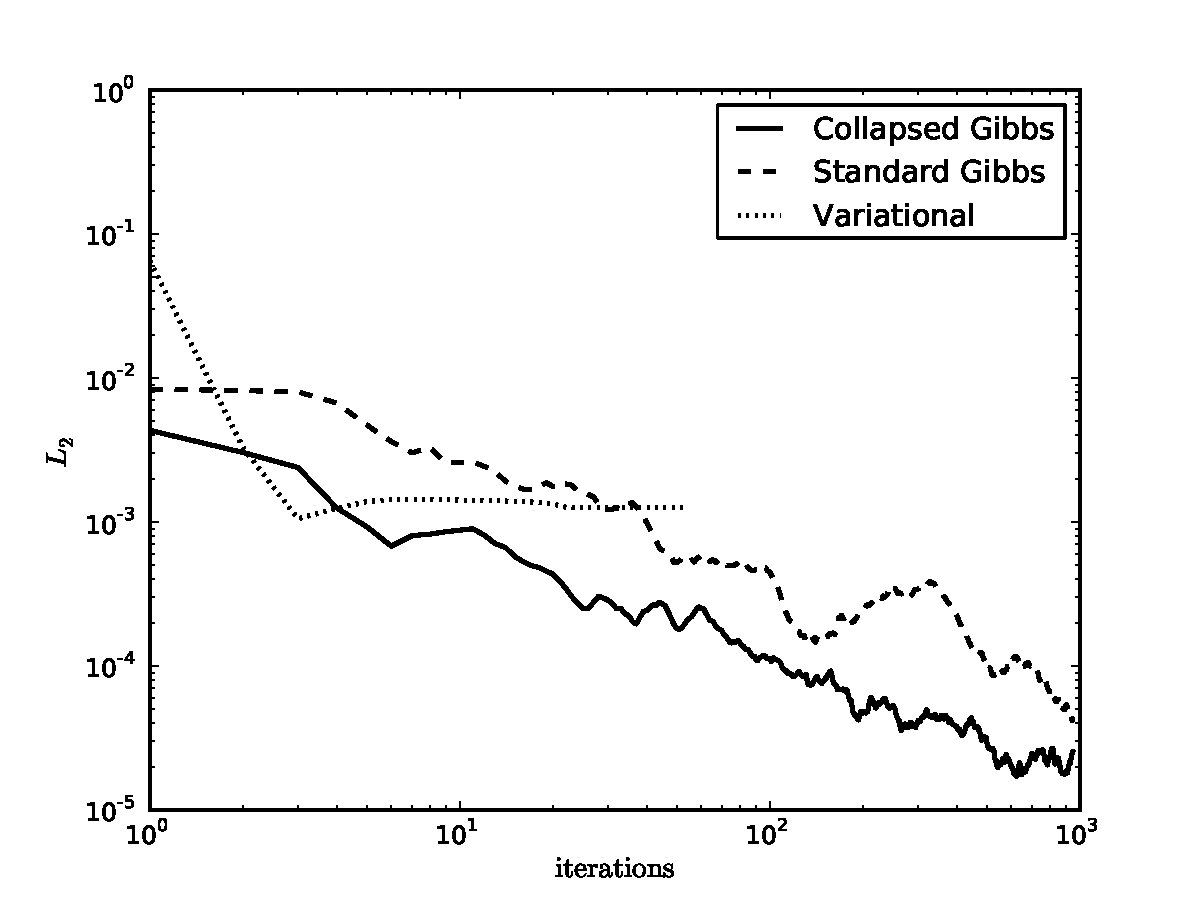
\includegraphics[width=0.9\textwidth]{../results.pdf}
    \caption{\figlabel{results}}
\end{figure}

\newpage

\section{Code} \label{sect:code}

\lstinputlisting[language=Python]{../lda.py}

\end{document}

